
%(BEGIN_QUESTION)
% Copyright 2012, Tony R. Kuphaldt, released under the Creative Commons Attribution License (v 1.0)
% This means you may do almost anything with this work of mine, so long as you give me proper credit

A FOUNDATION Fieldbus transmitter senses pressure inside a process vessel, through a liquid-filled capillary tube.  The height difference between the vessel connection point and the transmitter introduces a slight vacuum (negative pressure) at the transmitter's sensing port of -1.1 PSI due to the weight of the fill fluid.  The operators need to see the vessel's pressure displayed over a range of 0 to 58 PSI.  Determine the proper {\tt L\_type}, {\tt XD\_Scale}, and {\tt OUT\_Scale} values to enter into this transmitter's Analog Input function block when configuring the system:

$$\includegraphics[width=15.5cm]{i02134x01.eps}$$

\underbar{file i02134}
%(END_QUESTION)





%(BEGIN_ANSWER)

\begin{itemize}
\item{} {\tt L\_type} = Indirect
\item{} {\tt XD\_Scale} = -1.1 to 56.9 PSI 
\item{} {\tt OUT\_Scale} = 0 to 58 PSI
\end{itemize}

%(END_ANSWER)





%(BEGIN_NOTES)

{\bf This question is intended for exams only and not worksheets!}.

%(END_NOTES)


